\documentclass[a4paper,12pt,fleqn]{book}

% ---------------------------------------------------------------------------
%				Packages
% ---------------------------------------------------------------------------

% texdoc <nom_package> pour avoir des infos
\usepackage{etex}

\usepackage[utf8]{inputenc}						% Encodage français
\usepackage[frenchb]{babel}						% Mise en forme française
\usepackage[T1]{fontenc}						% Encodage caractères français

\usepackage{fourier}							% Différents symboles et polices
\usepackage[scaled=0.875]{helvet}				% Font générale
\usepackage{courier}							% Font télétype
\renewcommand{\ttdefault}{lmtt}					% Font télétype
\usepackage{frcursive}							% Ecriture manuscrite type écolier
\usepackage{calligra}							% Ecriture manuscrite classieuse
\usepackage{verbatim}							% Commentaires

\usepackage{amsfonts,amsmath,amssymb}			% Symboles maths
\usepackage{bm}									% Symboles maths en gras \bm{}
\usepackage{amstext}							% Texte en mode math de taille adaptée
\usepackage{amsopn}								% \DeclareMathOperator
\usepackage{mathrsfs}							% Symboles maths
\usepackage{mathtools}							% Symboles maths
\usepackage{theorem}							% Mise en forme des théorèmes

\usepackage{textcomp}							% Symboles
\usepackage{pifont}								% Symboles "ding"
\usepackage{wasysym}							% Symboles (smiley et logos)
\usepackage{epsdice}							% Symboles (faces d'un dé)
\usepackage[normalem]{ulem}						% Fioritures de texte (barré, etc...)
\usepackage{cancel}								% Barrer du texte (simplifier termes)
\usepackage{fancybox}							% Boîtes

\usepackage{tabularx}							% Tableaux évolués
\usepackage{diagbox}							% Cases en diagonale
%~ \usepackage{tabls}							% Espaces dans les tableaux (conflit avec bclogo)
\usepackage{colortbl}							% Coloration dans les tableaux
\usepackage{multirow}							% Fusionner les lignes d'un tableau
\usepackage{enumerate}							% Enumérations personnalisées
\usepackage{multicol}							% Environnement multicolonnes
\usepackage{fancyhdr}							% En-têtes et pieds de page
\usepackage[np]{numprint}					% Mise en forme des nombres

\usepackage[usenames, dvipsnames]{xcolor}		% Couleurs
\usepackage{graphicx}							% Insérer des images
\usepackage{pgf, tikz, tkz-tab, tkz-fct}		% Graphiques avec Tikz
\usetikzlibrary{arrows}
\usetikzlibrary{snakes}
\usepackage{alterqcm}							% QCM
\usepackage{circuitikz}							% Circuit éléctriques
\usepackage[tikz]{bclogo}						% Boites à logo

\usepackage{titlesec}							% Mise en forme des titres de sections
\usepackage{lastpage}							% Dernière page : \pageref{LastPage}

\usepackage{ifthen}								% Programmation conditions
\usepackage{multido}							% Boucles
\usepackage{calc}								% Calculs


\usepackage{etoolbox}
\makeatletter
\patchcmd{\ttlh@hang}{\parindent\z@}{\parindent\z@\leavevmode}{}{}
\patchcmd{\ttlh@hang}{\noindent}{}{}{}
\makeatother


\usepackage{listings}							% Listings
\lstset{literate=
	{á}{{\'a}}1 {é}{{\'e}}1 {í}{{\'i}}1 {ó}{{\'o}}1 {ú}{{\'u}}1
	{Á}{{\'A}}1 {É}{{\'E}}1 {Í}{{\'I}}1 {Ó}{{\'O}}1 {Ú}{{\'U}}1
	{à}{{\`a}}1 {è}{{\`e}}1 {ì}{{\`i}}1 {ò}{{\`o}}1 {ù}{{\`u}}1
	{À}{{\`A}}1 {È}{{\'E}}1 {Ì}{{\`I}}1 {Ò}{{\`O}}1 {Ù}{{\`U}}1
	{ä}{{\"a}}1 {ë}{{\"e}}1 {ï}{{\"i}}1 {ö}{{\"o}}1 {ü}{{\"u}}1
	{Ä}{{\"A}}1 {Ë}{{\"E}}1 {Ï}{{\"I}}1 {Ö}{{\"O}}1 {Ü}{{\"U}}1
	{â}{{\^a}}1 {ê}{{\^e}}1 {î}{{\^i}}1 {ô}{{\^o}}1 {û}{{\^u}}1
	{Â}{{\^A}}1 {Ê}{{\^E}}1 {Î}{{\^I}}1 {Ô}{{\^O}}1 {Û}{{\^U}}1
	{œ}{{\oe}}1 {Œ}{{\OE}}1 {æ}{{\ae}}1 {Æ}{{\AE}}1 {ß}{{\ss}}1
	{ű}{{\H{u}}}1 {Ű}{{\H{U}}}1 {ő}{{\H{o}}}1 {Ő}{{\H{O}}}1
	{ç}{{\c c}}1 {Ç}{{\c C}}1 {ø}{{\o}}1 {å}{{\r a}}1 {Å}{{\r A}}1
	{€}{{\euro}}1 {£}{{\pounds}}1 {«}{{\guillemotleft}}1
	{»}{{\guillemotright}}1 {ñ}{{\~n}}1 {Ñ}{{\~N}}1 {¿}{{?`}}1
}
\lstdefinestyle{customc}{
	belowcaptionskip=1\baselineskip,
	breaklines=true,
	frame=single,
	escapeinside={//!}{!},
	xleftmargin=\parindent,
	language=C,
	showstringspaces=false,
	basicstyle=\footnotesize\ttfamily,
	keywordstyle=\bfseries\color{green!40!black},
	commentstyle=\itshape\color{purple!40!black},
	identifierstyle=\color{blue},
	stringstyle=\color{orange!80!black},
}
\lstdefinestyle{custompy}{
	belowcaptionskip=1\baselineskip,
	breaklines=true,
	frame=single,
	escapeinside={//!}{!},
	xleftmargin=\parindent,
	language=python,
	showstringspaces=false,
	basicstyle=\footnotesize\ttfamily,
	keywordstyle=\bfseries\color{green!40!black},
	commentstyle=\itshape\color{purple!40!black},
	identifierstyle=\color{blue},
	stringstyle=\color{orange},
}
\lstdefinestyle{customjava}{
	belowcaptionskip=1\baselineskip,
	breaklines=true,
	frame=single,
	escapeinside={//!}{!},
	xleftmargin=\parindent,
	language=python,
	showstringspaces=false,
	basicstyle=\footnotesize\ttfamily,
	keywordstyle=\bfseries\color{green!40!black},
	commentstyle=\itshape\color{purple!40!black},
	identifierstyle=\color{blue},
	stringstyle=\color{orange},
}
\newcommand{\includecode}[2][c]{\lstinputlisting[style=custom#1]{#2}}
% ---------------------------------------------------------------------------
%				Macros simples (caractères)
% ---------------------------------------------------------------------------

\newcommand{\euro}{\eurologo{}}
\newcommand{\R}{\ensuremath{\mathbb{R}}}
\newcommand{\N}{\ensuremath{\mathbb{N}}}
\newcommand{\D}{\ensuremath{\mathbb{D}}}
\newcommand{\Z}{\ensuremath{\mathbb{Z}}}
\newcommand{\Q}{\ensuremath{\mathbb{Q}}}
\newcommand{\C}{\ensuremath{\mathbb{C}}}
\newcommand{\e}{\text{e}}
\renewcommand{\i}{\text{i}}
\newcommand{\s}{\ensuremath{\mathcal{S}}}
\newcommand{\sol}[1]{\mathcal{S}=\left\lbrace #1 \right\rbrace}
\newcommand{\ou}{\mbox{ ou }}
\newcommand{\et}{\mbox{ et }}
\newcommand{\si}{\mbox{ si }}
\newcommand{\Df}{\ensuremath{\mathcal{D}_f}}
\newcommand{\Cf}{\ensuremath{\mathcal{C}_f}}
\newcommand{\Dg}{\ensuremath{\mathcal{D}_g}}
\newcommand{\Cg}{\ensuremath{\mathcal{C}_g}}

\renewcommand{\P}{\ensuremath{\text{P}}}
\newcommand{\card}{\text{card}}
\newcommand{\E}{\text{E}}
\newcommand{\V}{\text{V}}

\newcommand{\FI}{\textbf{F.I.}}

\newcommand{\eq}{\ \Leftrightarrow\ } % ou \iff
\newcommand{\implique}{\Rightarrow}
\newcommand{\pheq}{\phantom{\eq}}
\newcommand{\egdef}{\stackrel{\textit{déf}}{=}}

\renewcommand{\ge}{\geqslant}
\renewcommand{\le}{\leqslant}
\newcommand{\supeg}{\geqslant}
\newcommand{\infeg}{\leqslant}

\newcommand{\lacco}{\left\lbrace}
\newcommand{\racco}{\right\rbrace}
\newcommand{\labs}{\left|}
\newcommand{\rabs}{\right|}

\newcommand{\inclus}{\subset}
\newcommand{\ninclus}{\not\subset}
\newcommand{\union}{\cup}
\newcommand{\inter}{\cap}

\newcommand{\non}[1]{\text{non(}#1\text{)}}

\newcommand{\dx}{~\text{d}x}
\newcommand{\dt}{~\text{d}t}

\renewcommand{\Re}{\text{Re}}
\renewcommand{\Im}{\text{Im}}
\newcommand{\conj}[1]{\overline{#1}}
\newcommand{\abs}[1]{|#1|}

\newcommand{\pinf}{+\infty}
\newcommand{\minf}{-\infty}
\newcommand{\pminf}{\pm\infty}

\newcommand{\para}{\ /\!\!/\ }

\newcommand{\comb}[2]{\text{C}_{#1}^{#2}}

\newcommand{\vect}[1]{\mathchoice
	{\overrightarrow{\displaystyle\mathstrut#1\,\,}}
	{\overrightarrow{\textstyle\mathstrut#1\,\,}}
	{\overrightarrow{\scriptstyle\mathstrut#1\,\,}}
	{\overrightarrow{\scriptscriptstyle\mathstrut#1\,\,}}}

\def\Oij{$\left(\text{O},~\vect{i},~\vect{j}\right)$}
\def\Oijk{$\left(\text{O},~\vect{i},~ \vect{j},~ \vect{k}\right)$}
\def\Ouv{$\left(\text{O},~\vect{u},~\vect{v}\right)$}

\newcommand{\vu}{\vect{u}}
\newcommand{\vv}{\vect{v}}
\newcommand{\vw}{\vect{w}}
\newcommand{\vn}{\vect{n}}

\newcommand{\veccol}[3]{\left(\begin{array}{c}
{#1}\\{#2}\\{#3}
\end{array}\right)}

\definecolor{gris}{gray}{0.85}
\newcommand{\surl}[1]{\colorbox{gris}{\textbf{#1}}}

\renewcommand{\emph}{\textbf}

\newcommand{\saut}{\ \\}
\newcommand{\lignesep}{\vspace*{5pt}\hrule\vspace*{5pt}}

\newcommand{\fct}[5]{
	\begin{array}[t]{r ccl}
	{#1}\ : \ &{#2}&\longrightarrow&{#3}\\
	&{#4}&\longmapsto&{#5}
	\end{array}}

\newcommand{\encadre}[1]{\fbox{\begin{minipage}{\textwidth}
#1
\end{minipage}}}

%\newcommand{\boite}[1]{\fbox{\Huge\phantom{A}\hspace*{#1}}}
\newcommand{\boite}[1]{\fbox{\rule[-0.2cm]{0pt}{0.6cm}\hspace*{#1}}}
\newcommand{\bboite}[1]{\fbox{\rule[-0.4cm]{0pt}{1cm}\hspace*{#1}}}

\newcolumntype{C}[1]{>{\centering\arraybackslash }m{#1}}

\newcommand{\espvert}[2]{\rule[-#1cm]{0cm}{#2cm}}

\newcommand{\suit}{\begin{tikzpicture}
\draw[color=white](-0.4em,0em)--(-0.25em,0em);
\draw ((-0.25em,-0.15em)--(0.07em,0.18em);
\draw (0.07em,0.18em) arc (135:0:0.25em);
\draw (0.5em,0em) arc (-180:-45:0.25em);
\draw (0.93em,-0.18em)--(1.36em,0.25em);
\draw (1.01em,0.25em)--(1.36em,0.25em)--(1.36em,-0.1em);
\draw[color=white](1.40em,0em)--(1.55em,0em);
\end{tikzpicture}}


%\newcommand{\suit}{\hookrightarrow}

% Commande programmation Casio

\newcommand{\touche}[1]{\fbox{\texttt{#1}}}

\newcommand{\toucheF}[2]{
$\underset{\text{\scriptsize F#2}}{\touche{#1}}$
}

\newcommand{\sto}{\ensuremath{\rightarrow}}

%\newcommand{\toucheFF}[2]{\begin{tabular}[t]{c}
%\touche{#1}\\
%{\scriptsize F#2}
%\end{tabular}}

\newcommand{\suiv}{$\vartriangleright$} % Menu suivant

\newcommand{\rl}{\begin{tikzpicture}[scale=0.7] % Retour à la ligne de la Casio
\draw[color=white] (0,0)--(0,0);
\draw [<-] (0.2em,0.2em)--(1em,0.2em)--(1em,0.8em);
\end{tikzpicture}}

\newcommand{\disp}{\begin{tikzpicture}[scale=0.7] % Triangle de la Casio
\draw[color=white] (0,0)--(0,0);
\fill (0.2em,0em)--(0.8em,0em)--(0.8em,0.8em)--(0.2em,0em);
\draw[color=white] (1em,1em)--(1em,1em);
\end{tikzpicture}}

\newcommand{\vers}{$\rightarrow$}

\newcommand{\enonce}{\textbf{Énoncé :}}
\newcommand{\solution}{\textbf{Solution :}}
\newcommand{\tq}{~,~}

\newcommand{\xmin}{x_{\text{min}}}
\newcommand{\xmax}{x_{\text{max}}}

% -------------------- Symboles : -------------------------------------------

\newcommand{\happy}{\smiley}
\newcommand{\sad}{\frownie}

\newcommand{\attention}{\danger}
\newcommand{\piege}{\bomb}
\newcommand{\interdit}{\noway}

\newcommand{\facede}[1]{\epsdice{#1}}

\newcommand{\hand}{\text{\ding{43}}}
\newcommand{\victory}{\text{\ding{44}}}

\newcommand{\trefle}{\text{\ding{168}}}
\newcommand{\carreau}{\text{\ding{169}}}
\newcommand{\coeur}{\text{\ding{170}}}
\newcommand{\pique}{\text{\ding{171}}}

\newcommand{\checkbox}{\text{\ding{114}}}
\newcommand{\checkedbox}{\text{\mbox{\ding{114}\hspace{-.7em}\raisebox{.2ex}[1ex]{\ding{51}}}}}

\newcommand{\scisors}{\ding{34}}
\newcommand{\couperici}{\scisors\dotfill\textit{\small{couper ici}}\dotfill\scisors}

% ---------------------------------------------------------------------------
% 				Environnements 
% ---------------------------------------------------------------------------

% ------------------------ Théorèmes ----------------------------------------

\theorembodyfont{\normalfont} \theoremstyle{break}



%\newcommand{\Ex}{\noindent\textbf{Exemple : }}
\newcommand{\Rappel}{\noindent\textbf{Rappel : }}

% ------------------------ Python --------------------------------------------

\newcounter{cptspace}
\newcommand{\tab}[1]{
	\setcounter{cptspace}{#1}
	\whiledo{\value{cptspace}>0}{
		\hspace*{0em}\hspace*{0em}
		\addtocounter{cptspace}{-1}}}

\newcommand{\prompt}{{>}{>}{>}\ }

\newenvironment{python}
	{\par\ttfamily\small\vspace{0.2cm}
	\setbox0=\hbox\bgroup
	\begin{minipage}{\textwidth}
	\vspace{0.2cm}
%	\begin{tabbing}
	}
	{\vspace{0.2cm}
%	\end{tabbing}
	\end{minipage}
	\egroup
    \fbox{\box0}
	\par\rmfamily\normalsize\vspace{0.2cm}\noindent
	}

\newenvironment{algo1}
	{\begin{center}\begin{tabular}{|>{\texttt\bgroup}l<{\egroup}|}
	\hline}
	{\hline
	\end{tabular}\end{center}
	}

%\newenvironment{python}
%	{\par\ttfamily\small\vspace{0.2cm}
%	\begin{bclogo}[couleurBord=black, arrondi = 0.1, logo={}, barre = none]{Code python :}
%%	\begin{minipage}{\textwidth}
%%	\vspace{0.2cm}
%	}
%	{%\vspace{0.2cm}
%%	\end{minipage}
%	\end{bclogo}
%	\par\rmfamily\normalsize\vspace{0.2cm}\noindent
%	}

\newcommand{\pyth}[1]{\texttt{#1}}

% -------------------------- Boites bclogo -----------------------------------
\newenvironment{warning}
	{\begin{bclogo}[couleurBord=black, arrondi = 0.1, logo = \bcattention]}%{\Large\attention}]}
	{\end{bclogo}}
	
\newenvironment{forbidden}
	{\begin{bclogo}[couleurBord=black, arrondi = 0.1, logo = \bcinterdit]}%{\Large\interdit}]}
	{\end{bclogo}}

% ---------------------------------------------------------------------------
% 				Raccoucis clavier
% ---------------------------------------------------------------------------

\newcommand{\fctsurI}[3]{
	Soit $#1$ la fonction définie sur $#3$ par $$#1(x)=#2$$}
	
\newcommand{\hp}{Hors programme}
\newcommand{\hpsti}{Hors programme de TSTI2D}
\newcommand{\hps}{Hors programme de TS}

% ---------------------------------------------------------------------------
%				Macros évoluées
% ---------------------------------------------------------------------------

% ----------------- \tournerpage --------------------------------------------
% Indique de tourner la page en bas de page
%
\def\tournerpage{\vfill%
	\begin{flushright}	
		\textbf{Tourner la page }$\mathbf{\rightarrow}$
	\end{flushright}
	\newpage}

% ------------------ Exercices : \exo et \pb --------------------------------
% Crée un exo (ou un pb) valant #1 points (si #1=0 alors correction)
% Les exos sont numérotés automatiquement
% 
\newcounter{numexo}
\setcounter{numexo}{0}

\newcommand\exo[1]{\addtocounter{numexo}{1}\par\vspace{1cm}\textbf{\textsc{Exercice \thenumexo}}%
	\ifthenelse{\equal{#1}{0}}{}{ \hfill \textbf{#1 points}}\medskip\par}
	
\newcommand\pb[1]{\par\vspace{1cm}\textbf{\textsc{Problème}}%
	\ifthenelse{\equal{#1}{0}}{}{\hfill \textbf{#1 points}}\medskip\par}

% ------------------ Cartouche : \makecartouche -------------------------------
% {Titre}{{Classe}{Durée}{Calculatrice autorisée}{Ligne pour le nom}
\newcommand{\calculatrice}{est }
\newcommand{\makecartoucheDsNOM}[4]{
	\ifthenelse{\boolean{#4}}{\renewcommand{\calculatrice}{est }}{\renewcommand{\calculatrice}{\textbf{n'est pas }}}
	\begin{center}\begin{tabular}{|p{.82\linewidth}|p{.15\linewidth}|}
	\hline
	#3 & \multicolumn{1}{r|}{#2}\\
	%~ \multicolumn{2}{|l|}{#3}\\
	% ----- Nom Prénom ----
	\hline
%	\textbf{\textsc{Nom - Prénom :}} & \textbf{\textsc{Classe :}}\\
	\multicolumn{2}{|l|}{\textbf{\textsc{Nom - Prénom :}}}\\
	\multicolumn{2}{|l|}{}\\
	\multicolumn{2}{|l|}{}\\
	% ---------------------
	\hline
	\multicolumn{2}{|c|}{}\\
	\multicolumn{2}{|c|}{\textbf{\LARGE{#1}}}\\
	\multicolumn{2}{|c|}{}\\
	\hline
	\multicolumn{2}{|c|}{\textit{La calculatrice \calculatrice autorisée. Aucun autre document n'est autorisé.}} \\
	\hline
	\end{tabular}\end{center}
}

\newcommand{\makecartoucheDsPASNOM}[4]{
	\ifthenelse{\boolean{#4}}{\renewcommand{\calculatrice}{est }}{\renewcommand{\calculatrice}{\textbf{n'est pas }}}
	\begin{center}\begin{tabular}{|p{.82\linewidth}|p{.15\linewidth}|}
	\hline
	#3 & \multicolumn{1}{r|}{#2}\\
	\hline
	\multicolumn{2}{|c|}{}\\
	\multicolumn{2}{|c|}{\textbf{\LARGE{#1}}}\\
	\multicolumn{2}{|c|}{}\\
	\hline
	\multicolumn{2}{|c|}{\textit{La calculatrice \calculatrice autorisée. Aucun autre document n'est autorisé.}} \\
	\hline
	\end{tabular}\end{center}
}

\newcommand{\makecartoucheDS}[5]{\ifthenelse{\boolean{#5}}{\makecartoucheDsNOM{#1}{#2}{#3}{#4}}{\makecartoucheDsPASNOM{#1}{#2}{#3}{#4}}}

\newcommand{\makecartoucheCours}[2]{
	\begin{center}\begin{tabular}{|p{.82\linewidth}|p{.15\linewidth}|}
	\hline
	 & \multicolumn{1}{r|}{#2}\\
	\hline
	\multicolumn{2}{|c|}{}\\
	\multicolumn{2}{|c|}{\textbf{\LARGE{#1}}}\\
	\multicolumn{2}{|c|}{}\\
	\hline
	\end{tabular}\end{center}
}


% --------------------------------- Pages de cahier ------------------------------

% --------------------- \cahierseyes ---------------------------------------------
% Crée une page de cahier réglures seyes (8mm et interlignes) de #1 lignes
%

% Périmé
\newcounter{dimcahierX}
\setcounter{dimcahierX}{16}
\newcounter{dimcahiersY}
\newcommand\Cahierseyes[1]{
	\vspace*{-1cm}
	\setcounter{dimcahiersY}{#1*\real{-0.8}}
	\begin{center}
	\begin{tikzpicture}
		\tkzInit[xmin=0,xmax=\thedimcahierX,ymin=\thedimcahiersY,ymax=0]
		\tkzGrid[xstep=0.8, ystep=0.8,sub, subxstep=0.8, subystep=0.2]
	\end{tikzpicture}
	\end{center}
}

% Bon
\newcounter{DimcahierX}
\setcounter{DimcahierX}{16}
\newcounter{DimcahierY}
\newcommand\cahierseyes[1]{
%	\vspace*{-0.8cm}
	\setcounter{DimcahierY}{#1}
	\begin{center}
	\begin{tikzpicture}
	\draw[xstep=0.8cm, ystep=0.2cm, color=lightgray] (0,0) grid (\theDimcahierX, 0.8*\theDimcahierY);
	\draw[xstep=0.8cm, ystep=0.8cm, color=gray] (0,0) grid (\theDimcahierX, 0.8*\theDimcahierY);
	\end{tikzpicture}
	\end{center}
}


% --------------------- \cahierpetca ---------------------------------------------
% Crée une page de cahier petits carreaux (5mm) de #1 lignes
%

%Périmé
%\newcounter{dimcahierpcY}
%\newcommand\cahierpetca[1]{
%	\setcounter{dimcahierpcY}{#1*\real{0.5}}
%	\vspace*{-1cm}
%	\begin{center}
%	\begin{tikzpicture}
%		\tkzInit[xmin=0,xmax=\thedimcahierX,ymin=0,ymax=\thedimcahierpcY]
%		\tkzGrid[xstep=0.5, ystep=0.5]
%	\end{tikzpicture}
%	\end{center}
%}

%Bon
\newcounter{DimcahierpcY}
\newcommand\cahierpetca[1]{
	\setcounter{DimcahierpcY}{#1}
	%\vspace*{-1cm}
	\begin{center}
	\begin{tikzpicture}
	\draw[xstep=0.5cm, ystep=0.5cm, color=gray] (0,0) grid (\theDimcahierX, 0.5*\theDimcahierpcY);
	\end{tikzpicture}
	\end{center}
}

\newcommand\Cahierpetca[1]{\cahierpetca{#1}}

% --------------------- \cahierligne ---------------------------------------------
% Crée une page de cahier avec juste des lignes (10mm) de #1 lignes
%
\newcounter{dimcahierlY}
\newcounter{miX}
\setcounter{miX}{\thedimcahierX*\real{0.5}}
\newcommand\cahierligne[1]{
	\setcounter{dimcahierlY}{#1-1}
	\begin{center}
	\begin{tikzpicture}
		\tkzInit[xmin=0,xmax=\thedimcahierX,ymin=0,ymax=#1]
		\foreach \k in {0,1,...,\thedimcahierlY}
		{\draw[color=gray] (0,\k)--(16,\k);}
		\draw[color=lightgray] (\themiX,0)--(\themiX,#1);
	\end{tikzpicture}
	\end{center}
}

% --------------------- \cahier ---------------------------------------------
% Par défaut, réglures seyes
%
\newcommand\cahier[1]{\cahierseyes{#1}}

% --------------------- \papiermilli ----------------------------------------
% Crée une feuille de papier millimétré de dimensions x=#1 par y=#2
%
\newcommand\papiermilli[2]{
	\begin{center}
	\begin{tikzpicture}
		\tkzInit[xmin=0,xmax=#1,ymin=0,ymax=#2]
		\tkzGrid[color=lightgray,xstep=1, ystep=1,sub, subxstep=0.1, subystep=0.1]
		\tkzGrid[color=gray,xstep=1, ystep=1,sub, subxstep=0.5, subystep=0.5]
		\tkzGrid[color=darkgray,xstep=5, ystep=5]
	\end{tikzpicture}
	\end{center}
}
% --------------------- \systlin ----------------------------------------
% Système linéaire 2*2
% Paramètres : a, ±b, c, a', ±b', c'
%
\newcommand{\systlin}[6]{
$\left\lbrace
\begin{array}{r @{x~} l @{y~=~} l l}
#1&#2&#3&(L_1)\\
#4&#5&#6&(L_2)
\end{array}
\right.$
}


% ---------------------------------------------------------------------------
%				Formatage
% ---------------------------------------------------------------------------

% --------------------- Chapitres -------------------------------------------
\addto\captionsfrench{\renewcommand{\chaptername}{~Chapitre}}

\titleformat{\chapter}[frame]
	{\vspace*{-2cm}\titleline[r]{}\normalfont}
	{\filright\texttt\LARGE{~\chaptername~\thechapter~}}
	{5pt}
	{\Huge\bfseries\scshape\filcenter}
	{}
	
%~ \titleformat{\chapter}[display]
%~ {\normalfont\Large\filcenter}
%~ {\titlerule[1pt]%
 %~ \vspace{1pt}%
 %~ \titlerule
 %~ \vspace{1pc}%
 %~ \LARGE{\chaptertitlename} \thechapter}
%~ {1pc}
%~ {\titlerule
 %~ \vspace{1pc}%
 %~ \Huge\bfseries}

% --------------------  Divisions logiques ----------------------------------

\setcounter{secnumdepth}{3} \setcounter{tocdepth}{3}
\renewcommand{\thepart}{Partie \arabic{part}}
\renewcommand{\thechapter}{\arabic{chapter}}
\renewcommand{\thesection}{\arabic{section}}
\renewcommand{\thesubsection}{\arabic{section}.\arabic{subsection}}
\renewcommand{\thesubsubsection}{\arabic{section}.\arabic{subsection}.\arabic{subsubsection}}

% -------------------- Numérotations des questions et puces -----------------

%\renewcommand{\theenumi}{\textbf{\arabic{enumi}}}
%\renewcommand{\labelenumi}{\textbf{\theenumi.}}
%\renewcommand{\theenumii}{\textbf{\alph{enumii}}}
%\renewcommand{\labelenumii}{\textbf{\theenumii.}}
%\renewcommand{\labelenumiii}{\textbullet}

\AtBeginDocument{\renewcommand{\labelitemi}{\textbullet}}
\AtBeginDocument{\renewcommand{\labelitemii}{\textbullet}}


% % -------------------- Mise en page --------------------------------------- 

\usepackage[francais]{layout}
%\usepackage[a4paper]{geometry}


% % -------------------- Réglages divers------------------------------------- 

\everymath{\displaystyle\everymath{}}		% Toutes les équations en mode \displaystyle
\DecimalMathComma							% Virgule comme séparateur décimal
\frenchspacing								% Espaces français
\setlength{\parindent}{0pt}					% Pas d'indentation de paragraphes

\colorlet{gris1}{black!20}
\colorlet{gris2}{black!30}

% ----------------------------------------------------------------------------

% =============================================================================
% 								FIN PREAMBULE
% =============================================================================


% -------------------- Cours --------------------
\renewcommand{\theenumi}{\arabic{enumi}}
\renewcommand{\labelenumi}{\theenumi)}
\renewcommand{\theenumii}{\alph{enumii}}
\renewcommand{\labelenumii}{\theenumii)}
\renewcommand{\labelenumiii}{\textbullet}

\setlength{\textwidth}{156truemm}  %largeur de texte
\setlength{\textheight}{220truemm} %longueur de texte
\setlength{\topmargin}{-0.8cm} %début de text
\setlength{\oddsidemargin}{2truemm}
\setlength{\evensidemargin}{2truemm}
\setlength{\baselineskip}{.2cm} 

\pagestyle{fancy}
\fancyhf{}
\renewcommand{\chaptermark}[1]{\markboth{\bsc{\chaptername~\thechapter{} : #1}}{}}
\renewcommand{\headrulewidth}{0pt}
\renewcommand \footrulewidth{.2pt}
\lhead[\textsl{\leftmark}]{}%{\textsl{\rightmark}}
\rhead[]{\textsl{\leftmark}}
%\lfoot{\texttt{maths.muller@gmail.com}}
%\cfoot{\textsc{}}
%\rfoot{\thepage/\pageref{LastPage}}

\newtheorem{Th}{Théorème}[chapter]
\newtheorem{Dem}{Démonstration}[chapter]
\newtheorem{DemBac}{Démonstration (démo Bac)}[chapter]
\newtheorem{Exmp}{Exemple}[chapter]
\newtheorem{Rem}{Remarque}[chapter]
\newtheorem{Def}{Définition}[chapter]
\newtheorem{Nota}{Notations}[chapter]
\newtheorem{Prop}{Propriété}[chapter]
\newtheorem{Exo}{Exercice}[chapter]
\newtheorem{App}{Application}[chapter]
\newtheorem{Cons}{Conséquence}[chapter]
\newtheorem{Ex}{Exemple}[chapter]
\newtheorem{Algo}{Algorithme}[chapter]
\newtheorem{Lemme}{Lemme}[chapter]


\lfoot[\thepage]{}
%\cfoot{\textsc{Titre}}
\rfoot[]{\thepage}


\renewcommand{\encadre}[1]{
	\begin{center}
		\fbox{\parbox{0.9\linewidth}{
				\medskip
				
				#1
				
				\medskip
		}}
	\end{center}	
}	

\usepackage{hyperref}

\begin{document}

\title{\Huge{\textsc{TétrisBot}}}
\author{\textsc{Frédéric Muller - Lionel Ponton}\\ \ \\ \small{Projet maths-infos du DU 2\up{ème} année - 2018-2019}\\ \ \\}


%\date{\small{\textit{Version 1.01}}}
%\date{\vfill \flushleft \textit{Description}}
\date{\vfill \textit{Licence Creative Common BY-NC-SA}}
\maketitle


\clearpage{\pagestyle{empty}\cleardoublepage}

\chapter*{Introduction}
\addcontentsline{toc}{chapter}{Introduction}

Ce projet a été réalisé entre novembre 2018 et mai 2019 dans le cadre du DU CCIE de l'université d'Aix-Marseille et, plus précisément, pour le module \og Projet mathématiques et informatique \fg{} sous la direction de M. Tristan Colombo. Le but est d'implémenter des agents qui jouent de manière autonome au célèbre jeu Tétris et d'essayer de les optimiser afin qu'ils y jouent le mieux possible.

\bigskip

La réalisation du projet s'est essentiellement déroulée en trois phases.

\bigskip

La première phase a consisté à la réalisation complète du moteur de jeu. Plutôt que de partir d'une base existante ou de reprendre un code \og tout fait \fg{}, nous avons entièrement programmé \og notre \fg{} version de Tétris en respectant (presque) toutes les règles officielles du jeu disponibles à l'adresse \href{https://tetris.fandom.com/wiki/Tetris_Wiki}{https://tetris.fandom.com/wiki/Tetris\_Wiki}. Nous avons choisi une conception orientée objet afin d'avoir un moteur offrant une grande adaptabilité pour les différents procédés d'optimisation.

Nous avons défini un mode \textit{humain} qui permet de jouer en utilisant le clavier pour déplacer et retourner les pièces comme dans un jeu de Tétris usuel et qui a permis de tester le moteur. Nous avons également programmé, dès la phase de conception du moteur, plusieurs agents simples:
\begin{itemize}
	\item un agent purement aléatoire qui joue totalement au hasard (et donc de façon catastrophique);
	\item un agent par filtrage qui choisit parmi les coups possibles celui qui est optimal selon différents critères possibles (créer le moins de trous possibles, créer le plus de lignes possibles, augmenter le moins possibles la hauteur des colonnes, etc.);
	\item un agent par évaluation de coups qui cherche à maximiser une fonction d'évaluation de qualité du coup dépendant de plusieurs variables pondérées par différents paramètres.
\end{itemize}

\bigskip

La deuxième phase à consister à implémenter une optimisation par algorithme génétique. Le but était de déterminer les \og meilleurs \fg{} paramètres pour l'agent par évaluation de coups.

Dans cette phase, différentes voies ont été envisagées pour ce qui est du codage choisi, du mode de sélection des \og parents \fg{}, du mode de reproduction et de création de la nouvelle génération.

Les résultats obtenus ont été très satisfaisants, avec des agents parvenant à jouer des centaines de milliers de pièces d'affilée. Certaines limitations sont cependant apparues notamment en raison du caractère aléatoire de la fonction d'évaluation de coups.

\bigskip

La troisième et dernière phase a consisté à implémenter une optimisation à l'aide d'apprentissage par renforcement (\textit{reinforcement learning}). Une longue période  de documentation et de maîtrise des concepts et des techniques a été nécessaire. 

Nous avons choisi d'implémenter un apprentissage mettant en jeu un Q-Learning par itération de fonctions de valeur. Cette méthode demande idéalement de pouvoir stocker une matrice modélisant tous les états et toutes les actions possibles pour l'agent pour chaque état. Ceci s'est avéré impossible pour un jeu présentant autant de configurations possibles que Tétris. En conséquence, nous avons décidé d'une part d'implémenter sur un jeu de pièces réduit à un seul domino plutôt que sur le jeu de Tétris usuel à 7 pièces et ensuite nous avons limités la phase d'apprentissage à un échantillon aléatoire d'états plutôt que d'essayer de stocker en mémoire tous les états possibles.

Nous obtenons un agent qui fonctionne mais dans un cadre assez limité.

Pour contourner ce problème, il est nécessaire de faire appel aux toutes dernières techniques d'apprentissage profond (\textit{Deep Learning}) utilisant notamment des réseaux de neurones. Ceci a été abordé sur le plan théorique et algorithmique mais sans être implémenté pour notre moteur.

\bigskip

Le plan de ce rapport reprend pour l'essentiel ces trois grandes phases. 

Dans la première partie, après avoir retracé l'historique de la genèse et du développement du jeu Tétris, nous décrivons les règles suivies, l'implémentation du moteur de jeu et des premiers agents. 

Dans la deuxième partie, nous présentons le fonctionnement général des algorithmes génétiques avec les différents choix possibles puis nous détaillons l'implémentation que nous avons mise en {\oe}uvre pour Tétris. 

Enfin, la troisième partie est consacré au reinforcement learning. Après avoir rappelé les bases mathématiques concernant les processus de décision markoviens qui conduisent aux équations de Bellman, nous présentons le principe général de Q-Learning par itérations de fonctions de valeur et l'implémentation que nous en avons fait sur un jeu simplifié. Nous terminons cette partie par une ouverture sur le deep-Q-Learning en détaillant, du point de vue théorique, comment les réseaux de neurones peuvent être utilisés pour \og apprendre \fg{} à un agent à jouer à un jeu qui, tel Tétris, présente beaucoup trop de configurations pour être stockées en mémoire.

\bigskip






\setcounter{tocdepth}{1}
\tableofcontents
\thispagestyle{fancy}


\part{Le moteur de jeu}
\chapter{Le jeu Tétris}

\section{L'origine du jeu}

Tétris a été créé par Alekseï Leonidovitch Pajitnov au milieu des années 1980. Il était alors chercheur au centre informatique Dorodnitsyn de l'Académie des Sciences Soviétique, un laboratoire de recherche et développement de l'Union Soviétique. Il y travaillait à la reconnaissance de la voix humaine par les ordinateurs et, à ses heures perdues, s'amuser à programmer des jeux. 

\begin{center}
	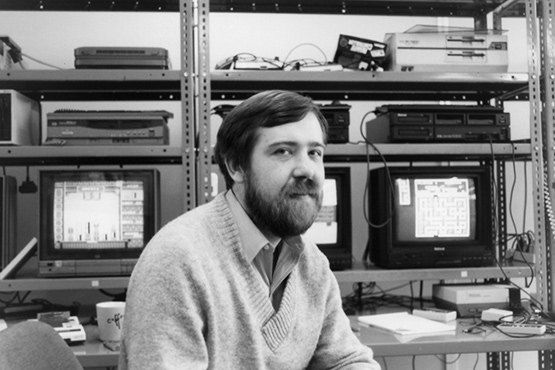
\includegraphics[scale=0.45]{media/Pajitnov.jpg}
	
	Alekseï Pajitnov
	
	(Source: \url{http://allrus.me/legendary-russian-game-programmer-alexey-pajitnov/})
\end{center}

Il avait entendu parlé d'un puzzle créé par le mathématicien américain Salomon Golomb, le \textit{pentomino}, dont le but était de recouvrir un rectangle avec des pièces de différentes formes, toutes obtenues par l'assemblage de 5 carrés identiques.

\begin{center}
	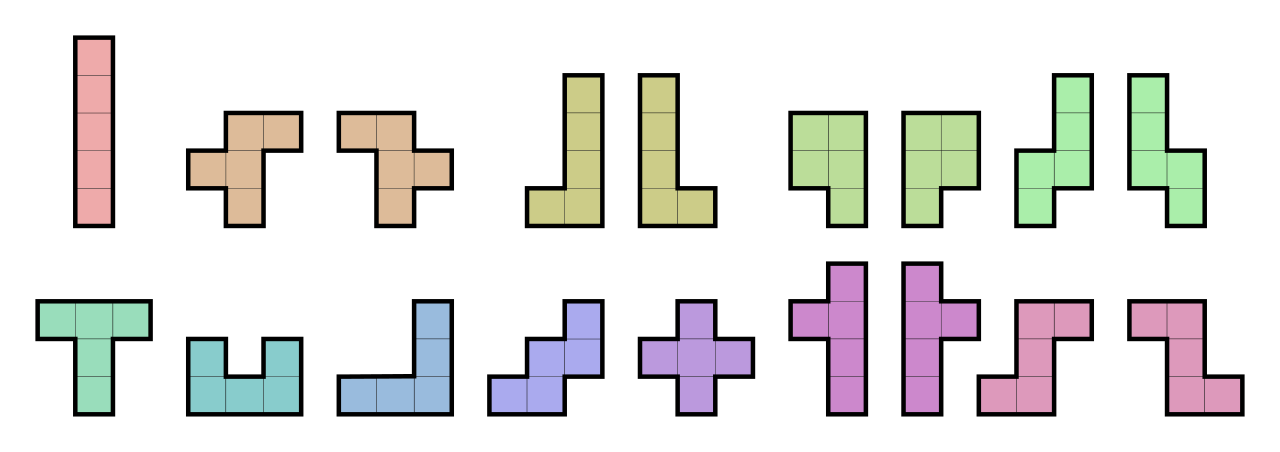
\includegraphics[scale=0.25]{media/pentomino.png}
	
	Les 18 pièces du Pentomino (en distinguant les pièces symétriques)
	
	(Source: \url{https://fr.wikipedia.org/wiki/Pentomino})
\end{center}


Il s'en procura un et, commençant à y jouer, découvrit que, malgré les apparences, ce n'était facile du tout! Il eut alors l'idée d'en faire un jeu électronique dans lequel les pièces étaient choisies aléatoirement, l'une après l'autre, et à des intervalles de temps de plus en plus réduits. Il fit des tests mais devant le (trop) grand nombre de combinaisons qu'offraient les 18 pièces du pentomino, il décida d'opter pour une version simplifiée dans laquelle il n'y aurait que 7 types de pièces, toutes formées à l'aide de 4 carrés identiques. Ces pièces sont nommées les \og tétraminos \fg{}\footnote{On trouve aussi les appellations \og tétrominos \fg{} ou \og tétriminos \fg{}.}, du grec \textit{tetra} qui signifie \textit{quatre}. 

\begin{center}
	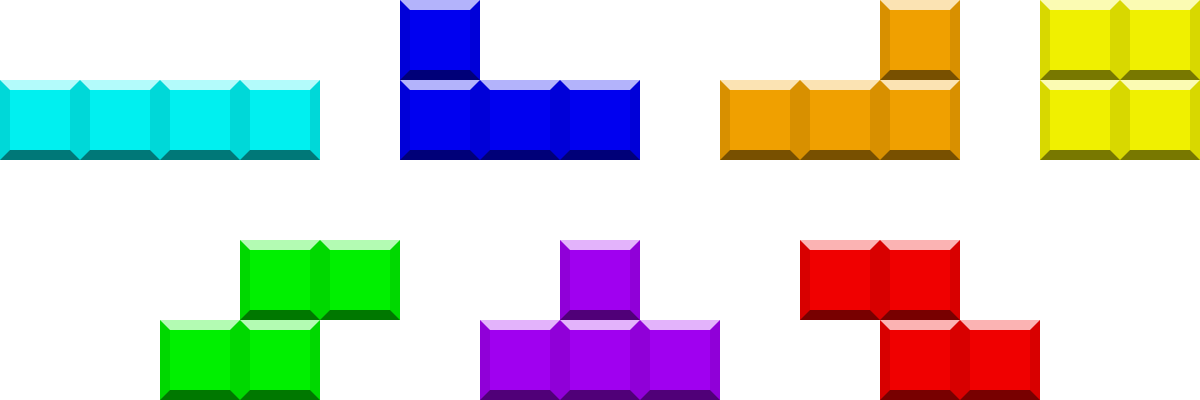
\includegraphics[scale=0.3]{media/tetromino.png}
	
	\medskip
	
	Les 7 tétraminos: I, J, L, O, S, T et Z.
	
	(Source: \url{https://en.wiktionary.org/wiki/tetromino})
\end{center}

Le jeu fut développé sur un Elektronica 60. Cet ordinateur ne disposait pas de fonctionnalités graphiques et les carrés formant les pièces furent alors représentés par un espace encadré de crochets: $[~]$.

\section{Le principe du jeu}

Le principe du jeu est le suivant: dans un champ de jeu rectangulaire, une pièce est choisie aléatoirement parmi les 7 tétraminos et se déplace du haut vers le bas. Le joueur peut faire tourner d'un, deux ou trois quarts de tour et déplacer horizontalement dans les deux sens la pièce afin de disposer le tétramino comme il le souhaite en bas du champ de jeu, sachant que les pièces successives s'empilent les unes sur les autres. Lorsque le joueur parvient à recouvrir une ligne complète du champ de jeu à l'aide de carrés des tétraminos, sans qu'il n'y ait plus aucun trou sur la ligne, celle-ci disparaît, rapportant un certain nombre de points, et la pile de tétraminos est décalée vers le bas, laissant ainsi plus de place dans le champ de jeu pour accueillir les pièces suivantes. Si, à un moment, le champ de jeu ne contient plus assez de place pour accueillir le tétramino suivant, la partie est perdue! Ainsi, Tétris n'est pas un jeu dans lequel une partie se termine par la victoire du joueur. Il s'agit plutôt de faire le meilleur score possible.

\begin{center}
	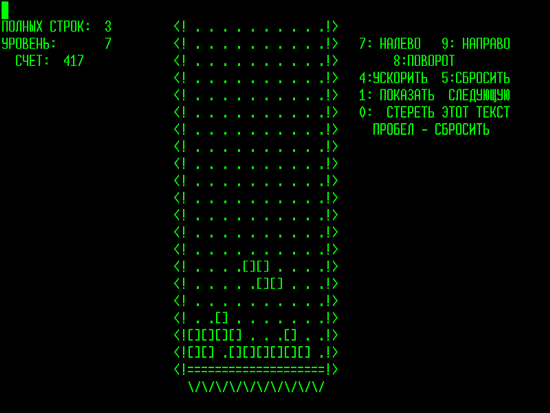
\includegraphics[scale=0.8]{media/premiere_version.png}
	
	Première version de Tetris 
	
	(Source: \url{https://www.firstversions.com/2015/11/tetris.html})
\end{center}

\section{Diffusion du jeu}

Sentant que le jeu serait plus attractif si les tétraminos apparaissaient \og véritablement \fg{} à l'écran plutôt que leur représentation à l'aide des crochets, Pajitnov décida d'améliorer l'aspect visuel de son programme grâce à une version pour PC d'IBM intégrant une interface graphique. Pour cela, il fit appel à un jeune lycéen prodige de 16 ans, Vadim Gerasimov, qui lui avait été présenté par un autre programmeur du nom de Dmitri Pavlovsky. Gerasimov avait des compétences qui dépassaient largement celles de Pajitnov et Pavlovsky: il avait notamment appris seul à programmer dans un langage venu de l'Ouest: le Microsoft DOS. \`A l'issue de deux mois de travail, Gerosimov créa la première version \og couleur \fg{} de Tétris qui intégrait également une table des meilleurs scores programmée par Pavlovsky.  Selon Vadim Gerasimov, le nom \textit{Tétris} résulte de la contraction des mots \og tétramino \fg{} et \og tennis \fg{}, ce dernier étant le sport favori de Pajitnov.


\begin{center}
	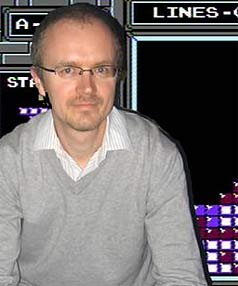
\includegraphics[scale=0.7]{media/Gerasimov.jpg}
	
	Vadim Gerasimov
	
	(Source:   \url{http://www.stuff.co.nz/technology/games/2477794/Tetris-inventor-makes-waves-at-Google})
\end{center}

Cette version se diffusa rapidement d'abord à Moscou puis dans les pays de l'ancien bloc soviétique. Une copie fut envoyée par Victor Brjabrin, le supérieur de Pajitnov, à l'Institut des Sciences Informatiques de Budapest où Robert Stein, un anglais d'origine hongroise travaillant pour une société de logiciels, découvrit le jeu. Stein vit le potentiel du jeu et envoya un fax au centre informatique Dorodnitsyn pour indiquer qu'il était intéressé par Tétris. Pajitnov lui répondit simplement qu'il était également intéressé et, à partir de cette simple réponse, Stein se mit à exploiter et vendre les droits de Tétris auprès de diverses compagnies occidentales, sans avoir signé le moindre accord avec les russes. Par la suite, il voulut établir un contrat en bonne et due forme avec Pajitnov et ses supérieurs mais ceux-ci étant confrontés à un monde inconnu pour eux, l'économie de marché, se montrèrent très méfiants et exigeants et les négociations n'aboutirent pas, ce qui n'empêcha pas Stein de continuer à exploiter le jeu. L'une des premières versions commerciales de Tétris fut celle éditée par Spectrum  Holobyte sur PC IBM en 1986. 

Par la suite, Elektronorgtechnica (abrégé ELORG), l'agence russe chargée de gérer les importations et exportations informatiques, repris le contrôle des négociations pour la gestion des droits et du marketing de Tétris, reprochant même à Pajitnov d'avoir donné un accord, fut-il de principe, à Stein, étant donné que, pendant l'ère soviétique, les créations intellectuelles des chercheurs russes étaient la propriété de l'état. Finalement, ELORG confirma l'accord avec Stein pour la gestion des droits du jeu mais seulement sur les ordinateurs et à l'exclusion de tout autre matériel électronique. 

En 1989, les droits d'exploitation restants furent partagés entre Atari pour les bornes d'arcade et Nintendo pour les consoles. Minuro Arakawa, le président de la filiale américaine de Nintendo avait mandaté Henk Rogers, afin d'obtenir ces droits car il comptait faire de Tétris l'un des jeux phare de sa nouvelle console: la Game Boy. Celle-ci fut mise sur le marché en 1989 et connue un succès phénoménal avec des millions d'exemplaires vendus à travers le monde. Si les ventes de la Game Boy participèrent à la diffusion de Tétris, celui-ci contribua également au succès de la console car le jeu était, dans un premier temps, implanté d'office sur la machine.

\begin{center}
	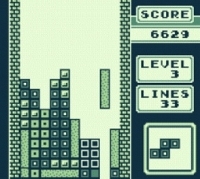
\includegraphics{media/Tetrisgb.jpg}
	
	Le jeu Tétris sur Game Boy en 1989
	
	(Source: \url{ https://de.wikipedia.org/wiki/Liste_der_erfolgreichsten_Computerspiele})
\end{center} 

Par la suite, Nintendo développa différentes variantes du jeu puis, après de l'effondrement de l'URSS en 1991, Pajitnov émigra aux \'Etats-Unis et récupéra finalement l'intégralité des droits de son jeu en 1996. Il fonda, avec Henk Rogers, The Tetris Compagny qui a depuis la charge exclusive de la gestion des droits du jeu. Ainsi, Pajitnov, qui n'a touché aucun droit d'auteur durant plus de 10 ans, peut aujourd'hui récolter les fruits de sa création.

\section{Les raisons du succès}

Tétris possède deux caractéristiques qui en font un modèle de jeu vidéo et qui peuvent expliquer son succès: d'une part, il est facile à prendre en main mais, dans le même temps, il possède un côté addictif et, d'autre part, malgré son apparente simplicité, il ne peut exister que sur un support électronique. Le principe du jeu fait qu'il procure une satisfaction quasi immédiate puisqu'on arrive très rapidement à supprimer une première ligne, puis une deuxième, etc... Il fait partie de la famille des \og jeux occasionnels \fg{} (\textit{casual gaming}) car une partie ne demande pas un gros investissement en terme de temps et on peut y jouer quelques minutes puis arrêter pour refaire une partie plus tard sans n'avoir rien perdu de significatif. 

Le choix de Pajitnov de réduire le nombre de pièces à 7 est également un élément déterminant. En effet, 7 est le nombre d'\og objets\footnote{Il faut comprendre ici le mot \textit{objets} dans un sens très large: images, mots, idées, nombres, etc...} \fg{} différents que l'esprit humain peut mémoriser rapidement et sans trop d'effort alors qu'à partir de 8, cela devient beaucoup plus difficile. Ainsi, 7 est le nombre idéal de pièces puisqu'elles peuvent être mémorisées rapidement par le joueur. 

Enfin, la simplicité de son programme et le peu de ressources qu'il requiert lui a permis d'être développé sur tous les supports de jeu successifs (ordinateur, borne d'arcade, console, smartphone...) 

\section{Peut-on gagner à Tétris?}
La principale difficulté dans Tétris est l'accélération de l'arrivée des nouvelles pièces qui devient vite difficilement gérable. Il est clair que si cette accélération continue indéfiniment, on atteint un palier au-delà duquel le jeu n'est plus jouable, ne serait-ce que parce que le temps de déplacement de la nouvelle pièce devient inférieur au temps matériellement nécessaire pour la déplacer à l'aide des touches de la console ou de l'ordinateur. 

Imaginons qu'on mette de côté cet aspect du jeu et que les pièces arrivent à intervalle régulier. Dans ce cas, peut-on gagner à Tétris? Telle quelle, la question n'a pas beaucoup de sens puisque le jeu ne prend fin qu'avec la défaite du joueur. Dans son mémoire de master, J. Brzustowski \cite{Bru92} étudie la question sous l'angle suivant: existe-t-il une stratégie qui permette de jouer à Tétris indéfiniment. Il montre que cela dépend essentiellement du choix aléatoire des pièces. En particulier, il prouve que, quelle que soit la stratégie adoptée, il existe une suite de tétraminos S et Z qui conduit inéluctablement à la fin de la partie. 

Notons, cependant, que, dans le cas d'un choix au hasard des tétraminos, la probabilité qu'une telle suite sorte est très faible. De plus, Brzustowski met en évidence que le jeu n'est pas programmé pour faire perdre le joueur par le choix des tétraminos. C'est d'ailleurs le contraire puisque, dans la spécification officielle du jeu (\textit{Guideline}) disponible sur le site de The Tetris Compagny\footnote{\url{http://tetris.wikia.com/wiki/Tetris_Guideline}}, il est précisé que les pièces sont en fait choisies par vague de 7, une vague consistant en une permutation quelconque des 7 tétraminos: c'est le principe du \og sac aléatoire \fg{} (\textit{random bag}). Dans cette configuration, des stratégies gagnantes sont possibles mais Brzustowski constate également que face à la réalité du jeu (i.e. en tenant compte des contraintes temporelles), l'expérience acquise pas un joueur est plus efficace qu'une stratégie mathématique prédéfinie.





%\chapter{Le jeu Tétris}

\section{Histoire}



\section{Règles du jeu adaptées au projet}


\chapter{Implémentation du moteur de jeu}

\section{Structures de données}
Le moteur de jeu est construit autour de trois classes :
\begin{itemize}
	\item \pyth{Tetramino} : les blocs 
	\item \pyth{Board} : la grille de jeu
	\item \pyth{TetrisEngine} : le moteur de jeu qui fait le lien entre les deux classes précédentes
\end{itemize} 

\section{La classe Tetramino}
La classe \pyth{Tetramino} est responsable de le gestion des blocs et de leurs rotations. Elle est implémentée dans le fichier \pyth{tetramino.py}.

Un bloc est défini par :
\begin{itemize}
	\item Un \pyth{id} qui permet d'identifier son type
	\item Un glyphe de base qui représente la pièce sans rotation dans une matrice carrée. Chaque case occupée par le bloc est codée par son \pyth{id} et les cases vides par 0.
	\item Le nombre de rotations (par exemple le O n'a qu'une seul rotation, le I en a deux et le T en a quatre)
\end{itemize}



\section{La classe Board}

\section{La classe TetrisEngine}


\chapter{Les agents}
Les agents sont à la base du projet dont le but est, justement, de les programmer.

\section{Généralités}
Un agent est essentiellement une classe qui a accès à un moteur de jeu (et donc à tous les paramètres de jeu) et qui implémente une méthode \pyth{getMove()} qui renvoie la commande du prochain coup à jouer. \\
C'est de leur responsabilité de lancer la partie.

Les fonctionnalités de base des agents sont implémentées dans la classe \pyth{Agent} dont les agents héritent tous. cette classe permet de :
\begin{itemize}
	\item Récupérer les paramètres de la grille après qu'un coup ait été joué via la méthode \pyth{getMoveStats(self, move)}. Cette méthode est utilisée dans la méthode \pyth{allMoveStats(self)} qui remplit un dictionnaire dont les clefs sont les différents placements possibles et les valeurs un dictionnaire content les différentes statistiques de jeu (nombre de lignes créées, nombre de trous,...)
	\item Créer une commande pour un placement direct via la méthode \pyth{commandFromMove(self, move)}.
\end{itemize}

\section{Joueur humain en mode texte}
Pour tester les différentes fonctionnalités du moteur, nous avons implémenté un agent, \pyth{AgetHuman}, qui se contente de recevoir les différentes commandes à jouer via l'entrée standard.\\
Grâce à cet agent nous avons pu tester le déplacement et la rotation des pièces, la suppression des lignes,...

\section{Agent aléatoire}
Ensuite le premier agent automatique qui joue de manière aléatoire. \\
\pyth{AgentRandom1} joue des coups aléatoires de type "aller à gauche", "tourner la pièce",... à la manière d'un joueur humain.\\
\pyth{AgentRandom2}, quant à lui, place directement les pièces dans des colonnes et des rotations aléatoires.\\

Évidemment ces deux agents sont catastrophiques en terme de performances mais ne demandent qu'à être améliorés (ces sont les "hello world" des agents).

\section{Agent par filtrage}
Le premier agent un tant soit peu efficace.\\
La stratégie utilisée est de filtrer la liste des coups jouables successivement selon plusieurs critères :
\begin{itemize}
	\item D'abord il ne garde que les coups qui font le moins de trous
	\item Ensuite, parmi eux, il ne garde que ceux qui donnent une somme des hauteurs des colonnes de la structure minimal
	\item Puis, ceux qui minimisent le bumpiness
	\item Enfin sont qui créent le plus de lignes 
\end{itemize} 

Cet agent joue plutôt bien pour une heuristique aussi simple.

\section{Agent par évaluation des coups}
Cet agent est à la base de ce que nous ferons avec les algorithmes génétiques :\\
Pour chaque coup jouable notons $L$ le nombre de lignes, $H$ la somme des hauteurs des colonnes, $T$ le nombre de trous créés et $B$ le bumpiness, après que le coup ait été joué.\\
La qualité d'un coup peut être évaluée par une fonction $$f(L,H,T,B)=a\times L - b\times H - c\times T - d\times B$$
où $a$, $b$, $c$ et $d$ sont des paramètres positifs que nous pouvons supposés dans $[0~;~1[$ (en effet on pourrait, sans perte de généralité les diviser par $a+b+c+d$ pour s'y ramener si ce n'était pas le cas).\\

Le coup à jouer est donc celui qui maximise cette fonction.\\

Tout le problème consiste à déterminer ces coefficients et c'est le but de l'optimisation par algorithme génétique.



\part{Optimisation par algorithmes génétiques}


\part{Optimisation par reinforcement learning}





\end{document}
